\chapter{Opgaveformulering}

%Her indsættes den konkrete opgaveformulering som I selv har udarbejdet på baggrund af et evt. projekt oplæg.

Konstruer et system der via en PC serielt kommunikerer med en hovedenhed. PC'en er afhængig af et login for at benytte alle funktioner. Dette login kommer fra en kodelås, hvis kode skal være korrekt, som har direkte kontakt til hovedenheden. Hovedenheden benytter via en powerline, X10 kommunikation. Denne kommunikation har til opgave at aktivere/deaktivere ønskede 230Vac udtag. Disse udtag har til opgave at sikre huset og specielt børn for farer. Dette kan f.eks gøres vha. en magnet lås til en køkkenskuffe.   
Ydermere skal hovedenheden via PC'en kunne udsende en SMS, hvis babyalarmen aktiveres.

Nedenstående figur \ref{fig:Systemoversigt} illustrer ovenstående.

\begin{figure}[htbp]
  \centering
    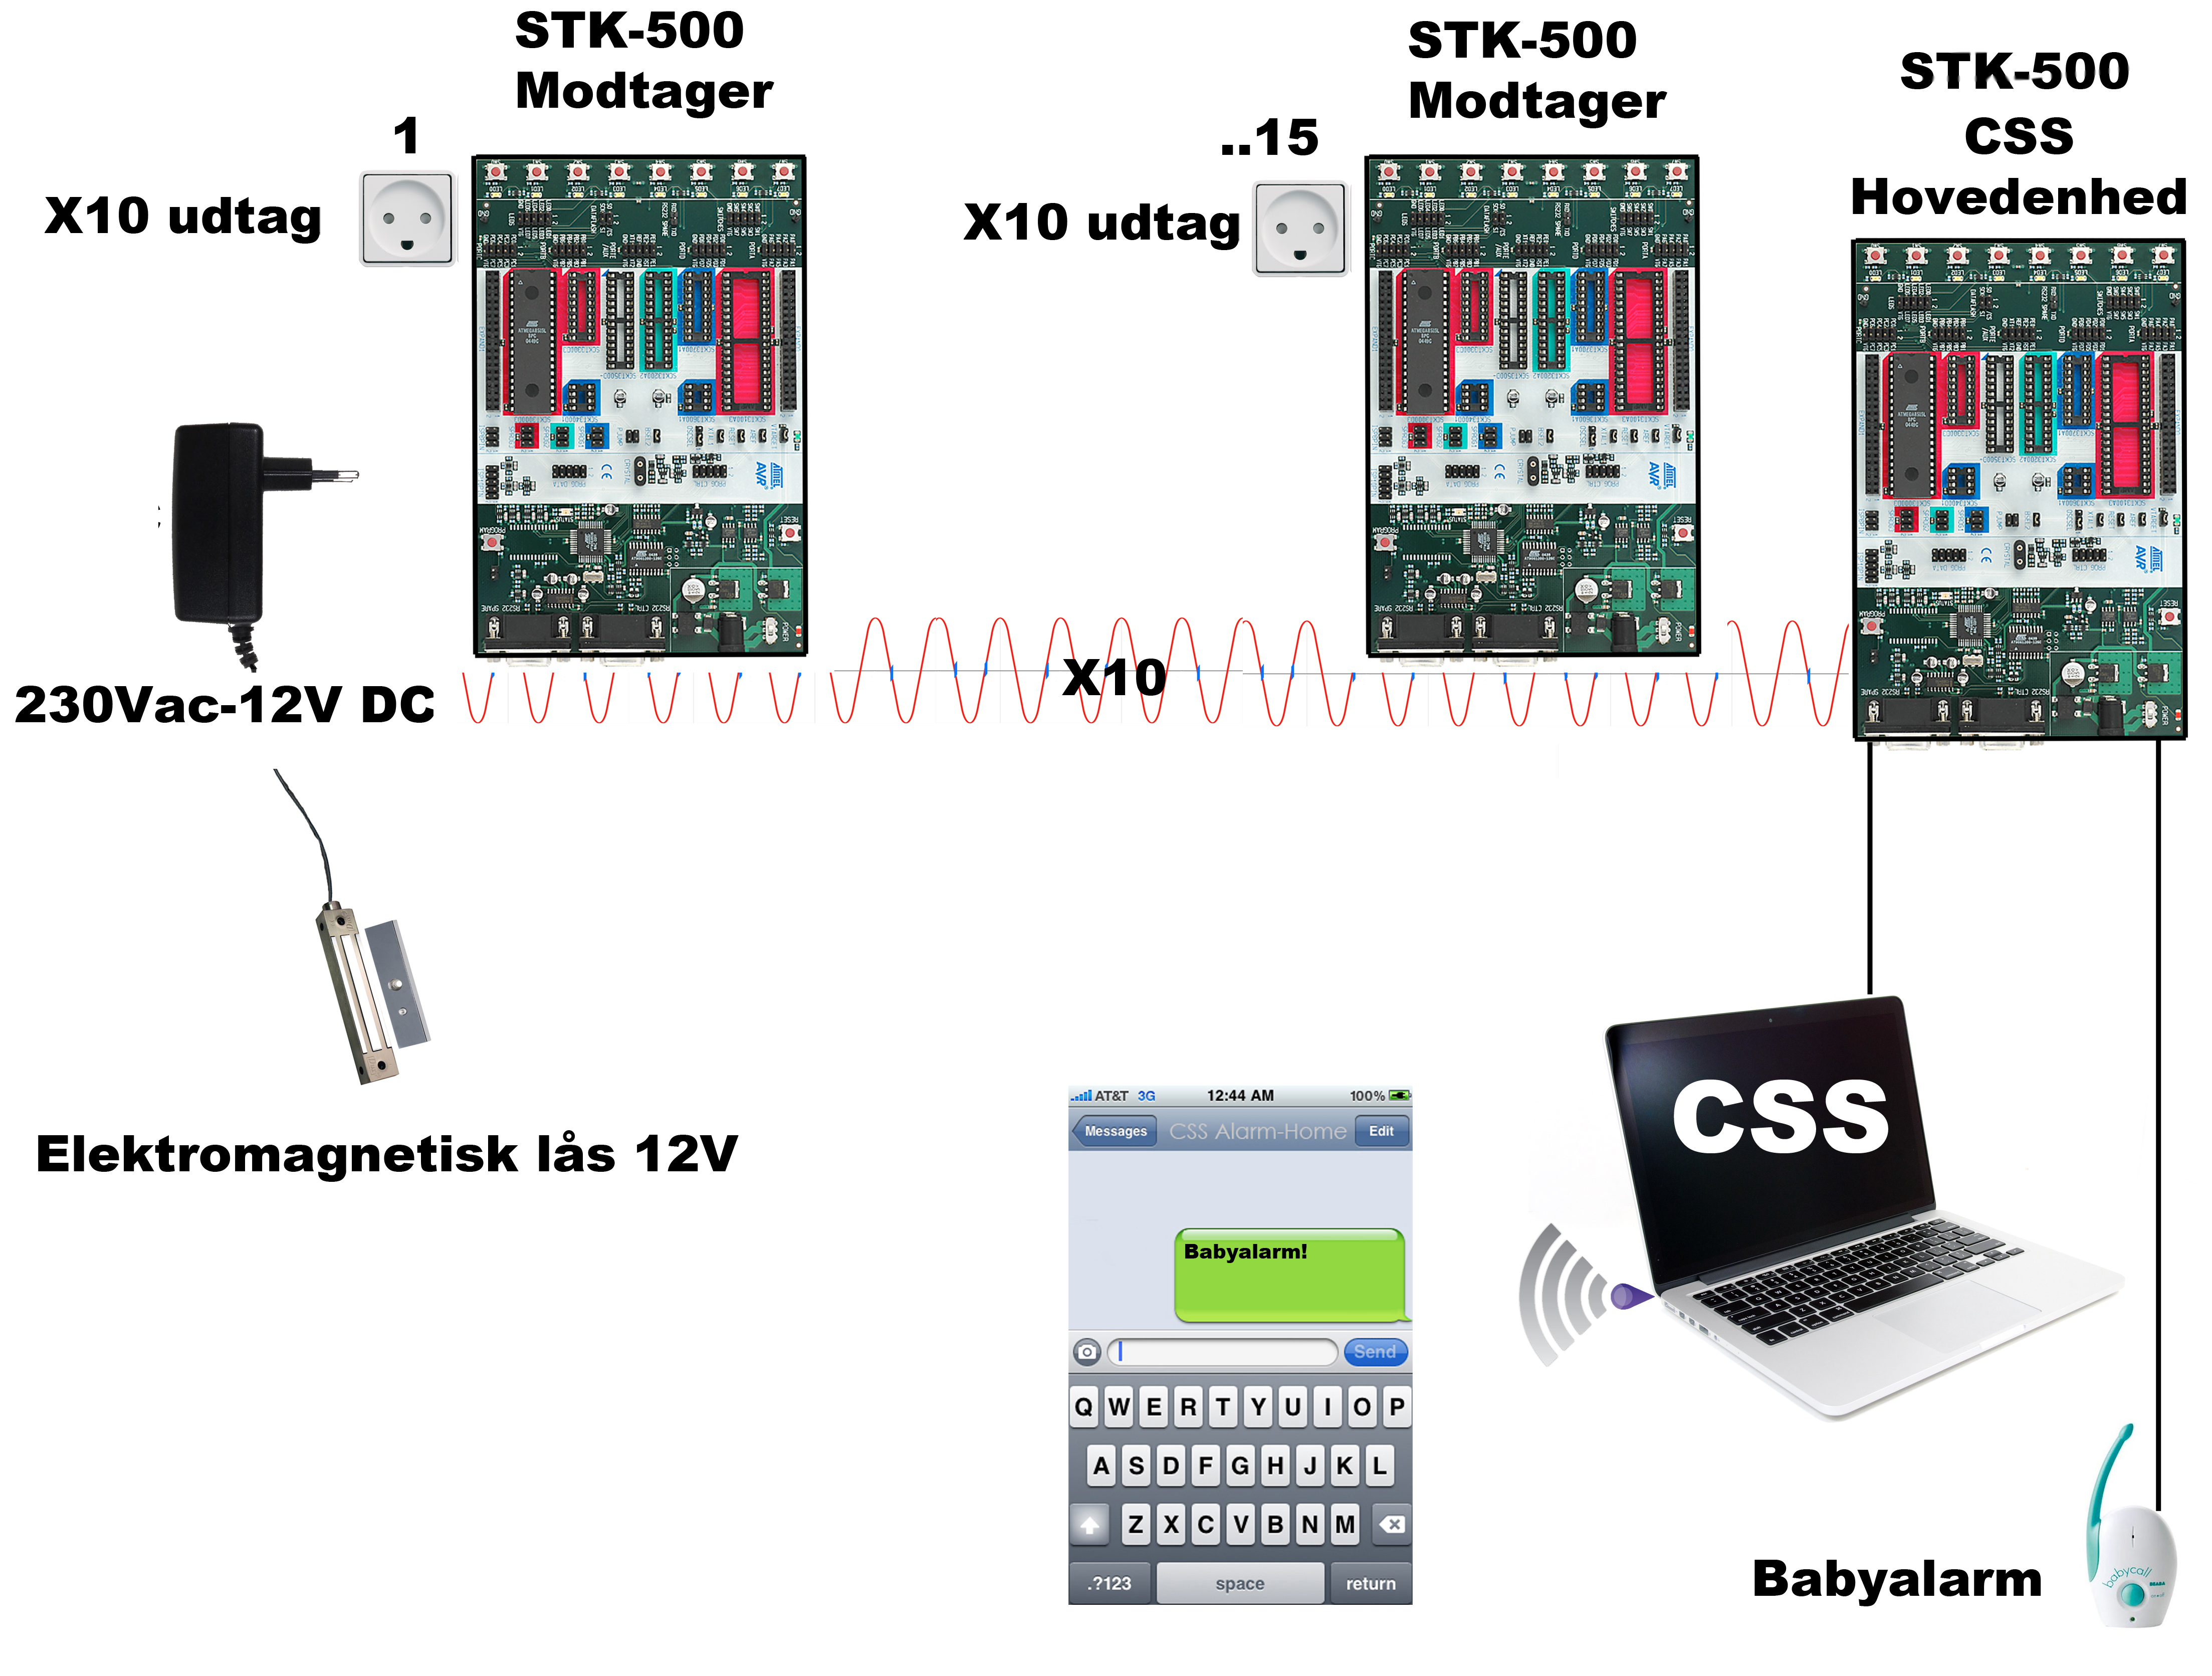
\includegraphics[width=0.8\textwidth]{billeder/Oversigt.png}
    \caption{Systemoversigt}
    \label{fig:Systemoversigt}
\end{figure}